\newpage
\section{Mehansko nihanje in valovanje}
\subsection{Enostavna nihala - enačba (dušenega) nihanja}
\subsubsection*{Utež na vijačni vzmeti}
\begin{center}
    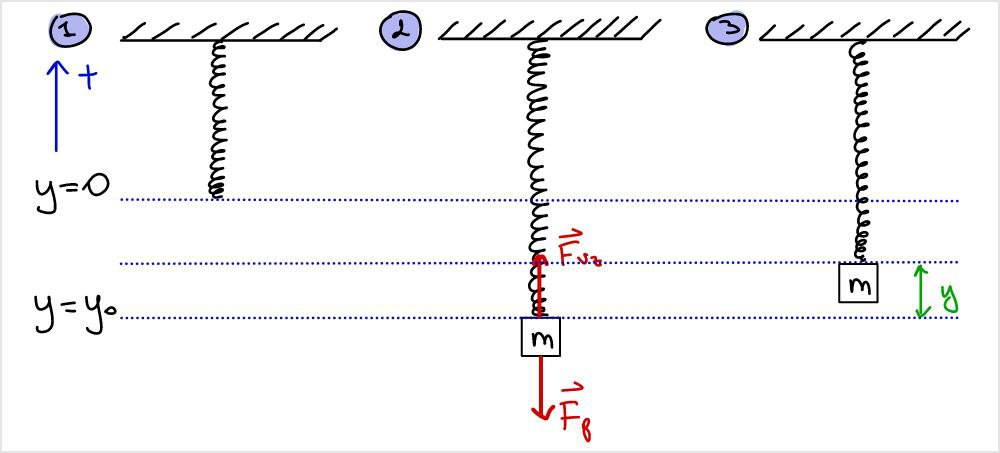
\includegraphics[width=0.7\textwidth]{img/01_001.jpg}      
\end{center}

\begin{enumerate}
    \item Vzmet je neraztegnjena.
    \item Obesimo vzmet z utežjo mase \(m\). Izračunamo \(y_0\) (ravnovesno lego):
    \begin{itemize}
        \item Zapišemo sile, ki delujejo na utež:
        \begin{enumerate}
            \item[(1)] Sila teže: \(\vec{F}_\text{g} = \vc{0}{-mg_0}{0}\), kjer je \(g_0 = 10 \, m / s^2\) težni pospešek;
            \item[(2)] Sila vzmeti: \(\vec{F}_\text{vz} = \vc{0}{-ky_0}{0}\), kjer je \(k > 0\) koeficient vzmeti.
        \end{enumerate}
        \item Zapišemo II.\ Newtonov zakon:
        \[
        \vec{a} = 0 \iff \vec{F} = m \vec{a} = 0 \implies \vec{F}_\text{g} + \vec{F}_\text{vz} = 0.
        \]
        Torej 
        \[
        -mg_0 - ky_0 = 0 \implies mg_0 = -ky_0 \implies y_0 = -\frac{mg_0}{k} \quad \textcolor{red}{(*)}
        \]        
    \end{itemize}
    \item Zdaj odmikamo utež od ravnovesne lege. Izračunamo \(y = y(t)\):
    \begin{itemize}
        \item Utež ima hitrost v smeri \(y\): \( v_y = \dot{y} = \frac{dy}{dt} \neq 0\).
        \item Zapišemo sile, ki delujejo na utež:
        \begin{itemize}
            \item[(1)] Sila teže: \(\vec{F}_\text{g} = -mg_0 \widehat{e}_y\), kjer je \(\widehat{e}_y\) enotski vektor;
            \item[(2)] Sila vzmeti: \(\vec{F}_\text{vz} = -ky\widehat{e}_y\);
            \item[(3)] Sila upora: \(\vec{F}_\text{u} = -C \vec{v} = -C \dot{y} \widehat{e}_y\). Sila upora se pojavi, ker nismo v vakuumu.
        \end{itemize}
        \item Zapišemo II.\ Newtonov zakon:
        \begin{itemize}
            \item \(\vec{F} = \vec{F}_\text{g} + \vec{F}_\text{vz} + \vec{F}_\text{u}\);
            \item \(\vec{F} = m \vec{a} = m \ddot{y} \widehat{e}_y\).
        \end{itemize}
        Torej 
        \[
        -C \dot{y} \widehat{e}_y - ky\widehat{e}_y -mg_0 \widehat{e}_y = m \ddot{y} \widehat{e}_y \implies 
        \left( \ddot{y} + \frac{C}{m} \dot{y} + \frac{k}{m} y + g_0 \right) \widehat{e}_y = 0 \implies 
        \ddot{y} + \frac{C}{m} \dot{y} + \frac{k}{m} y + g_0 = 0.
        \]
        \item Vpeljemo oznake \(\beta := \frac{C}{m}, \ [\beta]  = s^{-1}; \ \omega_0^2 := \frac{k}{m}, \ [\omega_0^2] = s^{-2}\). Dobimo enačbo:
        \[
        \ddot{y} + \beta \dot{y} + \omega_0^2 y + g_0 = 0.
        \]
        \item Iz \(\textcolor{red}{(*)}\) sledi, da \(g_0 = -\frac{k}{m}y_0 = - \omega_0^2y_0\).  
        \df{Enačba dušenega nihanja} je:
        \[
        \ddot{y} + \beta \dot{y} +  \omega_0^2 (y - y_0) = 0.
        \]        
    \end{itemize}
\end{enumerate}

\begin{opomba}
    Enačba \(\ddot{y} + \beta \dot{y} + \omega_0^2y = \omega_0^2 y_0\) je 
    \begin{itemize}
        \item Diferencialna enačba 2.\ reda za \(y\).
        \item Linearna (členi \(y, \ \dot{y}, \ \ddot{y}\) imajo 1.\ potenco).
        \item Koeficienti so konstantni (niso odvisni od časa).
        \item Pogojno nehomogena (lahko jo spravimo v homogeno enačbo).
    \end{itemize}
\end{opomba}

\paragraph{Postopek reševanja enačbe dušenega nihanja}
\begin{enumerate}
    \item Definiramo \(y' := y - y_0\). S tem enačba postane homogena.
    \item Enačbo rešujemo z nastavkov \(y' = A e^{\lambda t}\), kjer sta \(A, \ \lambda\) neki konstanti, \([\lambda] = s^{-1}, \ [A] = m\). 
    
    Dobimo karakteristični polinom \(\lambda^2 + \beta \lambda + \omega_0^2 = 0\).
    \item Karakteristični polinom ima diskriminanto \(D = \beta^2 - 4 \omega_0^2\). Definiramo \(\omega^2 := \omega_0^2 - \left(\frac{\beta}{2}\right)^2\). Dobimo \(D = - 4 \omega^2\). Ločimo možnosti.
\end{enumerate}

\textbf{(a) \(D < 0 \ (\omega^2 > 0)\)}. V tem primeru dobimo \df{podkritično dušenje}.

Splošna rešitev je \textcolor{red}{TODO (izpeljava)}
\[
    y' = \exp\left(-\frac{\beta}{2}t\right) (A_1 \exp(i\omega t) + A_2 \exp(-i\omega t)) = \exp\left(-\frac{\beta}{2}t\right)(B_1 \cos(\omega t) + B_2 \sin(\omega t)) = B \exp\left(-\frac{\beta}{2}t\right) \sin (\omega t + \delta),
\]
kjer je \(\delta\) \df{fazni zamik}.


